% ACL 2026 EvalEval Workshop paper — Complete Rewrite
% compile: pdflatex acl_latex && bibtex acl_latex && pdflatex acl_latex && pdflatex acl_latex

\documentclass[11pt]{article}
\usepackage[review]{acl}

% Standard packages
\usepackage{times}
\usepackage{latexsym}
\usepackage[T1]{fontenc}
\usepackage[utf8]{inputenc}
\usepackage{microtype}
\usepackage{inconsolata}
\usepackage{graphicx}
\usepackage{amsmath}
\usepackage{booktabs}
\usepackage{multirow}
\usepackage{xcolor}
\usepackage{tikz}
\usepackage{enumitem}
\usepackage{pifont}
\usepackage{url}
\newcommand{\cmark}{\ding{51}}
\usetikzlibrary{positioning, arrows.meta, shapes.geometric}

% Tighten floats
\setlength{\floatsep}{4pt plus 2pt minus 2pt}
\setlength{\textfloatsep}{6pt plus 2pt minus 2pt}
\setlength{\intextsep}{4pt plus 2pt minus 2pt}

\title{Why LLM Leaderboards Are Incomparable:\\Structural Fragmentation and Missing Evaluation Metadata at Scale}

\author{Anonymous Author(s)\\
  EvalEval @ ACL 2026 Shared Task}

\begin{document}
\maketitle

% ===================================================================
\begin{abstract}
% ===================================================================
When the same model scores 16.67 on GPQA from one leaderboard and
49.0 from another---a 32-point gap---can we tell which number to
trust? We show systematically that we cannot. By ingesting
\textbf{29,331} evaluation records from \textbf{11~sources}
(8~leaderboards, model cards, and a paper-results archive) into the
standardised Every Eval Ever (EEE) schema, covering 5,672 models and
180 benchmarks, we find:
\textbf{(1)~Attribution failure}: among the 8~genuinely independent
cross-source collision pairs (the remaining 8 are likely copied
scores), all involve different harnesses and score gaps of up to
32~points, yet the metadata needed to explain these gaps---prompt
template, temperature, chain-of-thought---is absent in every case.
\textbf{(2)~Missing metadata}: prompt template and temperature are
documented in fewer than 0.1\% of records; headline coverage figures
(e.g., 96.7\% for n-shot) are inflated by a single source
contributing 91\% of records---excluding it drops n-shot coverage
to 62\% and chain-of-thought to 1\%.
\textbf{(3)~Structural fragmentation}: only 16~collision pairs
exist---24\% of the $\sim$67 expected under random assignment
($z=-6.1$, $p<0.001$)---because sources evaluate almost entirely
non-overlapping model--benchmark combinations.
In short, the community cannot currently determine whether a 5-point
lead on a leaderboard reflects genuine model superiority or merely
a difference in how the evaluation was run. We release our dataset,
pipeline, and analysis code to support reproducible evaluation
research.
\end{abstract}

% ===================================================================
\section{Introduction}\label{sec:intro}
% ===================================================================

The rapid progress of large language models (LLMs) is charted
through \emph{benchmark leaderboards}: publicly ranked tables of
accuracy, pass@$k$, or ELO scores on tasks such as MMLU
\citep{hendrycks-2021-mmlu}, GSM8K \citep{cobbe-2021-gsm8k}, or
HumanEval \citep{chen-2021-humaneval}. When Model~A scores 75\% and
Model~B scores 70\% on the same benchmark, the community treats it as
evidence that A outperforms B. But ``the same benchmark'' hides a
multitude of implementation choices---and changing those choices can
shift scores by 15 or more percentage points
\citep{alzahrani-2024-benchmarks}.

To understand why this happens, we need to decompose what a
\emph{benchmark result} actually consists of. A single published
score is the product of at least five independent decisions, which we
call the \textbf{evaluation context}:
%
\begin{enumerate}[leftmargin=2em, itemsep=1pt]
\item The \textbf{benchmark} itself: a dataset and a scoring rubric
  (e.g., ``MMLU with accuracy'').
\item The \textbf{evaluation harness}: the software framework that
  orchestrates tokenisation, generation, and scoring
  (e.g., lm-evaluation-harness, HELM, AlpacaEval).
\item The \textbf{n-shot count}: how many labelled exemplars are
  prepended to the prompt (e.g., 0-shot vs.\ 5-shot).
\item The \textbf{prompt template}: the exact formatting of the
  input—-how the question, choices, and exemplars are arranged in the
  model's context window.
\item The \textbf{generation configuration}: decoding strategy
  (greedy vs.\ sampling), temperature, top-$p$, and chain-of-thought
  reasoning.
\end{enumerate}
%
When evaluation reports omit these details---or when two sources use
the same \emph{benchmark name} but different underlying
configurations---scores that appear comparable become silently
incommensurable.

\citet{alzahrani-2024-benchmarks} demonstrate this concretely:
evaluating LLaMA~65B on MMLU produces a 14.9-point gap (63.7 vs.\
48.8) depending solely on whether HELM or lm-evaluation-harness is
used. Published leaderboards carry no warning of
such discrepancies.

Despite these well-documented case studies, no prior work has
measured how pervasive the problem is across the public evaluation
ecosystem: how many cross-source comparisons are structurally
possible, and what fraction carry sufficient metadata for
attribution.

\paragraph{This paper.}
We test four hypotheses about the state of the LLM evaluation
ecosystem:
%
\begin{description}[leftmargin=1.5em, itemsep=2pt, style=unboxed]
\item[\textbf{H1} (Metadata gap):] Critical evaluation-context
  metadata---prompt template, temperature, generation
  configuration---is largely absent from public evaluation artifacts,
  preventing attribution of cross-source score differences.
\item[\textbf{H2} (Structural fragmentation):] The current ecosystem
  is structurally fragmented: sources evaluate non-overlapping
  model--benchmark combinations, producing far fewer cross-source
  comparisons than would be expected under random assignment.
\item[\textbf{H3} (Attribution failure):] Even where cross-source
  collisions exist, the observed score differences cannot be
  attributed to specific evaluation-context choices because the
  required metadata is missing.
\item[\textbf{H4} (Pipeline fragility):] Even schema-valid
  ingestion pipelines produce semantically invalid records at
  non-trivial rates, requiring post-hoc auditing to distinguish
  genuine evaluation results from extraction artefacts.
\end{description}
%
To test these hypotheses, we build a modular, source-agnostic
pipeline that converts heterogeneous evaluation artifacts---8
leaderboard APIs, HuggingFace model cards, and the Papers With Code
archive---into the standardised Every Eval Ever (EEE) schema
\citep{evaleval-2026}. The pipeline comprises 11~dedicated converters
(publicly released) with shared schema validation and deduplication,
producing a unified dataset of 29,331 records covering 5,672 models
and 180 benchmarks. We provide the first systematic, cross-source
quantification of structural fragmentation and metadata coverage in
the LLM evaluation ecosystem, together with an empirical taxonomy
of extraction artefacts that schema validation alone cannot catch.

% ===================================================================
\section{Key Concepts}\label{sec:definitions}
% ===================================================================

\paragraph{Evaluation record and harness.}
An \emph{evaluation record} is a single JSON document conforming to
the EEE schema (v0.2.1) that captures one model's result on one
benchmark from one source, including four blocks:
\texttt{model\_info}, \texttt{eval\_library} (harness),
\texttt{source\_metadata}, and \texttt{evaluation\_results}.
The \emph{evaluation harness} is the software framework that
orchestrates prompting, generation, and scoring; different harnesses
can produce different scores for the same model on the same
benchmark because they differ in tokenisation, prompt formatting,
and answer extraction \citep{biderman-2024-lessons}.
We identify 11~distinct harnesses (Table~\ref{tab:sources}).

\paragraph{Structural wall.}
We use this term to describe the phenomenon where sources that
\emph{could} be compared (they measure the same constructs) cannot
\emph{actually} be compared because they evaluate non-overlapping
model subsets. This is not a metadata problem---it is a data
collection problem that no amount of documentation can fix.

\begin{table}[t]
\centering
\small
\setlength{\tabcolsep}{3pt}
\caption{Mapping between the five evaluation-context axes discussed
in this paper and the corresponding EEE schema fields. All reside
under \texttt{evaluation\_results[].generation\_config}.}
\label{tab:terminology}
\begin{tabular}{lll}
\toprule
\textbf{Concept} & \textbf{EEE field} & \textbf{Example} \\
\midrule
Harness        & \texttt{eval\_library.name}    & lm\_eval \\
Harness ver.   & \texttt{eval\_library.version} & v0.4.2 \\
N-shot         & \texttt{generation\_args.n\_shot} & 5 \\
Prompt tpl.    & \texttt{generation\_args.prompt\_template} & mcq\_v2 \\
Temperature    & \texttt{generation\_args.temperature} & 0.0 \\
Chain-of-thought & \texttt{additional\_details.cot} & True \\
\bottomrule
\end{tabular}
\end{table}

% ===================================================================
\section{Related Work}\label{sec:related}
% ===================================================================

\paragraph{Benchmark sensitivity.}
\citet{alzahrani-2024-benchmarks} show that leaderboard rankings are
sensitive to implementation details, with score gaps of up to 15
points on MMLU from harness choice alone.
\citet{biderman-2024-lessons} identify prompt format, tokenisation,
and generation configuration as key reproducibility axes and
recommend that evaluation reports surface these choices.
\citet{polo-2024-tinybenchmarks} demonstrate that a 100-item subset
of MMLU preserves ranking order under consistent evaluation
conditions---but this property breaks under methodology divergence.

\paragraph{Evaluation infrastructure.}
The two dominant open harnesses---lm-evaluation-harness
\citep{gao-2021-framework} and HELM \citep{liang-2022-holistic}---differ
in their defaults for n-shot count, answer normalisation, and prompt
template. Three newer platforms address metadata tracking:
LightEval \citep{fourrier-2024-lighteval} bundles prompt format,
metric, and shot count into version-controlled task templates;
OpenCompass \citep{contributors-2023-opencompass} tracks per-run
metadata across hundreds of tasks; and EKA-EVAL
\citep{kim-2025-ekaeval} adds cross-lingual coverage.
Crucially, all three operate as \emph{integrated} harnesses that
enforce metadata only for evaluations run within their own
pipelines---they provide no mechanism for comparing results
across platforms or against scores reported in papers and
leaderboards.

\paragraph{Documentation standards.}
Model cards \citep{mitchell-2019-modelcards} and datasheets
\citep{gebru-2021-datasheets} established documentation norms for
models and datasets; no analogous standard exists for evaluation runs.
MLPerf \citep{mattson-2020-mlperf} demonstrates that standardised,
auditable evaluation is feasible at industry scale but targets
hardware benchmarking, not the open-ended LLM evaluation ecosystem.

\paragraph{Positioning.}
Our work is the first \textbf{cross-source, multi-leaderboard,
schema-based quantification} of both structural fragmentation and
missing evaluation metadata.
\citet{alzahrani-2024-benchmarks} demonstrate that harness choice
alone shifts scores by up to 15 points---but only within a
controlled, single-benchmark experiment; we show that the public
ecosystem is too fragmented for such comparisons to arise
naturally at scale (16~collision pairs from 29,331~records).
\citet{biderman-2024-lessons} recommend documenting prompt format,
tokenisation, and generation configuration---but do not measure
how often the ecosystem actually follows this advice; we quantify
the gap ($<$0.1\% for prompt template and temperature).
Integrated harnesses (LightEval, OpenCompass, EKA-EVAL) enforce
metadata within their own pipelines but provide no mechanism for
comparing results across platforms; the EEE schema complements them
by standardising the \emph{reporting} of existing results from any
source, enabling the cross-platform collision analysis we present.

% ===================================================================
\section{Methodology}\label{sec:methodology}
% ===================================================================

\subsection{The EEE Schema}\label{sec:schema}

We adopt the EEE schema (v0.2.1) as-is, ensuring that our coverage
analysis reflects a community-endorsed standard rather than an
ad-hoc format \citep{evaleval-2026}. Each record contains four
blocks: \texttt{model\_info} (identity), \texttt{eval\_library}
(harness), \texttt{source\_metadata} (provenance), and
\texttt{evaluation\_results} (scores plus generation configuration).
A \emph{cross-source collision pair} $(m, b, s_1, s_2)$ arises
when model~$m$ is evaluated on benchmark~$b$ by two distinct
sources; we define the \emph{score delta} as
$\Delta = \text{score}_{s_1} - \text{score}_{s_2}$.
We define \emph{metadata coverage} for a field~$f$ as the fraction
of records where $f$ contains a non-trivial value (not empty, not
``unknown'').
The \texttt{generation\_config} fields
(Table~\ref{tab:terminology}) are first-class schema citizens, not
free-text notes, enabling the automated coverage analysis in
\S\ref{sec:coverage}.

\subsection{Data Collection Pipeline}\label{sec:pipeline}

The pipeline ingests each source via a dedicated \emph{converter}
module (source $\rightarrow$ EEE JSON $\rightarrow$ schema
validation $\rightarrow$ collision detection $\rightarrow$ coverage
analysis), with no shared mutable state between converters.
We ingest \textbf{8~leaderboard} sources
(OLv2, AlpacaEval~2, Chatbot Arena, BigCodeBench, EvalPlus, BFCL,
SWE-Bench, WildBench, MT-Bench) via dedicated APIs or HuggingFace
dataset downloads, \textbf{1~model-card} source (structured YAML
\texttt{model-index} from HuggingFace READMEs---benchmark-rich at
156~benchmarks but model-poor at 11~models), and \textbf{Papers
With Code} (576~records from 383~models across 16~benchmarks after
removing extraction artefacts and duplicates from an initial 1,350
raw records; \S\ref{sec:within}).

\subsection{Validation}\label{sec:validation}

Each source is implemented as an independent converter
(4~framework adapters, 7~leaderboard scrapers;
${\sim}4{,}900$~LOC; Appendix~\ref{app:converters}).
All 29,331~output records are validated against the EEE schema
(v0.2.1) via \texttt{jsonschema} (required fields, types, enum
constraints); duplicates are detected by composite key
\texttt{(model\_id, benchmark, source)}; and score sanity checks
flag values outside expected ranges (\S\ref{sec:within}).
For Papers With Code---the weakest source---we additionally
verified a sample of records against the original papers.

\subsection{Collision Detection}\label{sec:collision_method}

We define the collision detection procedure formally. Given a set of
evaluation records $R$, we:
%
\begin{enumerate}[leftmargin=2em, itemsep=1pt]
\item \textbf{Normalise} model identifiers: lowercase, strip
  \texttt{-hf} suffixes, unify separators (note that
  scraping-introduced typos---e.g., ``BlooombergGPT'' with a
  duplicated character---cannot be caught by rule-based
  normalisation and represent a lower bound on missed collisions).
\item \textbf{Normalise} benchmark names: lowercase, strip
  parenthetical shot annotations (e.g., ``GPQA (0-shot)''
  $\rightarrow$ ``gpqa''), unify separators.
\item \textbf{Group} records by (normalised model, normalised
  benchmark).
\item \textbf{Select} groups appearing in two or more distinct
  sources.
\item For each such group, emit all $\binom{k}{2}$ source pairs as
  collision pairs, annotated with score delta, harness match,
  n-shot match, and chain-of-thought match.
\end{enumerate}

% ===================================================================
\section{Results}\label{sec:results}
% ===================================================================

\subsection{Dataset Overview}

Table~\ref{tab:sources} summarises the 11 sources in our dataset.
The Open LLM Leaderboard v2 dominates with 91\% of records (26,790
of 29,331), reflecting its scale (4,465 models evaluated on 6
benchmarks using lm\_eval). The long tail of smaller sources---each
contributing 34--576 records---provides benchmark diversity (180
unique benchmarks) but limited model overlap.
Papers With Code is the least reliable source after cleaning:
of 1,350 raw records, 774 (57\%) were removed as extraction
artefacts or duplicates (\S\ref{sec:within}), yielding a 43\%
discard rate---the highest of any source and a concrete measure
of the data-quality challenges in cross-source ingestion.

\begin{table}[t]
\centering
\small
\setlength{\tabcolsep}{3pt}
\caption{Data sources in our dataset. ``Rec'' = evaluation records;
``Mod'' = unique models; ``Ben'' = unique benchmarks. Sources are
ordered by record count.}
\label{tab:sources}
\begin{tabular}{lrrrl}
\toprule
\textbf{Source} & \textbf{Rec} & \textbf{Mod} & \textbf{Ben} & \textbf{Harness} \\
\midrule
Open LLM LB v2   & 26,790 & 4,465 &   6 & lm\_eval \\
Papers w/ Code    &    576 &   383 &  16 & unknown \\
AlpacaEval 2      &    446 &   223 &   2 & alpaca\_eval \\
BFCL              &    327 &   109 &   3 & gorilla\_eval \\
BigCodeBench      &    280 &   156 &   2 & bigcodebench \\
Chatbot Arena     &    218 &   218 &   1 & fastchat \\
EvalPlus          &    214 &   125 &   2 & evalplus \\
HF Model Card     &    207 &    11 & 156 & varies \\
WildBench         &    122 &    61 &   2 & wildeval \\
SWE-Bench         &    117 &   117 &   1 & swebench \\
MT-Bench          &     34 &    34 &   1 & fastchat \\
\midrule
\textbf{Total}    & \textbf{29,331} & \textbf{5,672} & \textbf{180} & \textbf{11 distinct} \\
\bottomrule
\end{tabular}
\end{table}

\subsection{Metadata Coverage (H1)}\label{sec:coverage}

Table~\ref{tab:coverage} and Figure~\ref{fig:coverage} present the
coverage rates for five metadata fields across all sources.

\paragraph{The ecosystem without OLv2.}
Because Open LLM Leaderboard v2 contributes 91\% of records, headline
coverage figures are misleading. We therefore first present the
ecosystem \emph{excluding} OLv2 (Table~\ref{tab:ablation}, row~2):
across the remaining 2,541 records from 10~sources, n-shot coverage
is only \textbf{62.2\%}, chain-of-thought \textbf{1.1\%}, temperature
\textbf{0.2\%}, and prompt template \textbf{0.6\%}. Excluding both
OLv2 and PWC leaves 1,965 records where chain-of-thought,
temperature, and prompt template are all \textbf{0.0\%}. This is the
true state of the ecosystem: outside a single dominant source, nearly
all evaluation context metadata is absent.

\paragraph{Headline coverage (all sources).}
Two fields appear well-documented when OLv2 is included:
%
\begin{itemize}[leftmargin=1.5em, itemsep=1pt]
\item \textbf{N-shot count} (96.7\%): all leaderboard sources
  with few-shot benchmarks document it; the gap comes from
  sources where the concept does not apply (Chatbot Arena,
  WildBench, MT-Bench---all preference-based) and incompletely
  parsed model cards.
\item \textbf{Harness identity} (98\%): all dedicated leaderboard
  sources identify their evaluation framework; the 2\% gap comes from
  Papers With Code (harness genuinely unknown) and HF Model Cards
  (where harness detection dropped from 91\% to 32\% after we
  tightened parsing to exclude ambiguous identifiers).
  No source documents the harness \emph{version}---all
  29,331 records carry \texttt{eval\_library.version = "unknown"}
  because none of the ingested APIs, leaderboards, or model cards
  publish the framework release or commit hash.
  This is an ecosystem-wide gap, not a pipeline limitation.
\end{itemize}

Three fields are severely under-documented:
%
\begin{itemize}[leftmargin=1.5em, itemsep=1pt]
\item \textbf{Chain-of-thought} (76.3\%): documented only in Open
  LLM LB v2 (83.4\% of its records) and partially in Papers With
  Code (4.9\%). All other sources: 0\%.
\item \textbf{Temperature} ($<$0.1\%): only 6 of 29,331 records
  document temperature---all from Papers With Code.
\item \textbf{Prompt template} ($<$0.1\%): only 14~records contain
  prompt information (all from PWC). This is the most critical gap,
  because prompt formatting is the single most impactful
  undocumented axis of variation
  \citep{alzahrani-2024-benchmarks}.
  Even the 2.4\% figure for PWC is inflated: manual audit confirms
  that all 14~non-null \texttt{prompt\_template} values are
  extraction artefacts (variant tags and CoT labels), making the
  valid coverage rate 0\%.
  The true valid coverage for \texttt{prompt\_template} across all
  sources is therefore 0/29,331 (0.00\%)---the nominal $<$0.1\%
  figure is entirely an artefact false-positive rate of 100\%.
\end{itemize}

\paragraph{Sensitivity to source composition.}
Because Open LLM Leaderboard v2 contributes 91\% of records, the
headline coverage figures are dominated by this single source.
Table~\ref{tab:ablation} shows the effect of removing the two
largest sources. Without OLv2, n-shot coverage drops from 96.7\% to
62.2\%, and chain-of-thought coverage drops from 76.3\% to 1.1\%.
Excluding both OLv2 and PWC leaves 1,965 records from 9 sources
where n-shot coverage is 71.0\% but chain-of-thought, temperature,
and prompt template are all 0.0\%. This confirms that the few
well-documented fields depend almost entirely on a single source,
and the ecosystem-wide picture is starker than the headline numbers
suggest.

\begin{table}[t]
\centering
\small
\setlength{\tabcolsep}{3pt}
\caption{Sensitivity of metadata coverage to source composition.
Coverage rates (\%) under three ablations. The qualitative
pattern---temperature and prompt are absent---is stable, but n-shot
and CoT coverage depend heavily on OLv2.}
\label{tab:ablation}
\begin{tabular}{lrrrrr}
\toprule
\textbf{Subset} & \textbf{H} & \textbf{S} & \textbf{C} & \textbf{T} & \textbf{P} \\
\midrule
All (29,331)                &  98 & 96.7 & 76.3 & 0.0 & 0.0 \\
$-$\,OLv2 (2,541)          &  72 & 62.2 &  1.1 & 0.2 & 0.6 \\
$-$\,PWC (28,755)           & 100 & 98.0 & 77.7 & 0.0 & 0.0 \\
$-$\,OLv2$-$PWC (1,965)    &  93 & 71.0 &  0.0 & 0.0 & 0.0 \\
\bottomrule
\end{tabular}
\end{table}

\begin{table}[t]
\centering
\small
\setlength{\tabcolsep}{3pt}
\caption{Metadata documentation rates (\% of records with non-trivial
values) per source. Fields: H = harness, S = n-shot, C = chain-of-thought,
T = temperature, P = prompt template. Bold = 100\%.}
\label{tab:coverage}
\begin{tabular}{lccccc}
\toprule
\textbf{Source} & \textbf{H} & \textbf{S} & \textbf{C} & \textbf{T} & \textbf{P} \\
\midrule
Open LLM LB v2   & \textbf{100} & \textbf{100} & 83.4 & 0.0 & 0.0 \\
Papers w/ Code    &     0 & 32.1 & 4.9 & 1.0 & 2.4\footnotemark[1] \\
AlpacaEval 2      & \textbf{100} & \textbf{100} & 0.0 & 0.0 & 0.0 \\
BFCL              & \textbf{100} & \textbf{100} & 0.0 & 0.0 & 0.0 \\
BigCodeBench      & \textbf{100} & \textbf{100} & 0.0 & 0.0 & 0.0 \\
Chatbot Arena     & \textbf{100} &  0.0 & 0.0 & 0.0 & 0.0 \\
EvalPlus          & \textbf{100} & \textbf{100} & 0.0 & 0.0 & 0.0 \\
HF Model Card     &    32 &  5.8 & 0.0 & 0.0 & 0.0 \\
WildBench         & \textbf{100} &  0.0 & 0.0 & 0.0 & 0.0 \\
SWE-Bench         & \textbf{100} & \textbf{100} & 0.0 & 0.0 & 0.0 \\
MT-Bench          & \textbf{100} &  0.0 & 0.0 & 0.0 & 0.0 \\
\midrule
\textbf{Overall}  & \textbf{98} & \textbf{96.7} & \textbf{76.3} & \textbf{$<$0.1} & \textbf{$<$0.1} \\
\bottomrule
\end{tabular}
\end{table}
\footnotetext[1]{All 14 non-null values are extraction artefacts (variant tags and CoT labels); valid coverage is 0\%.}

\begin{figure}[t]
\centering
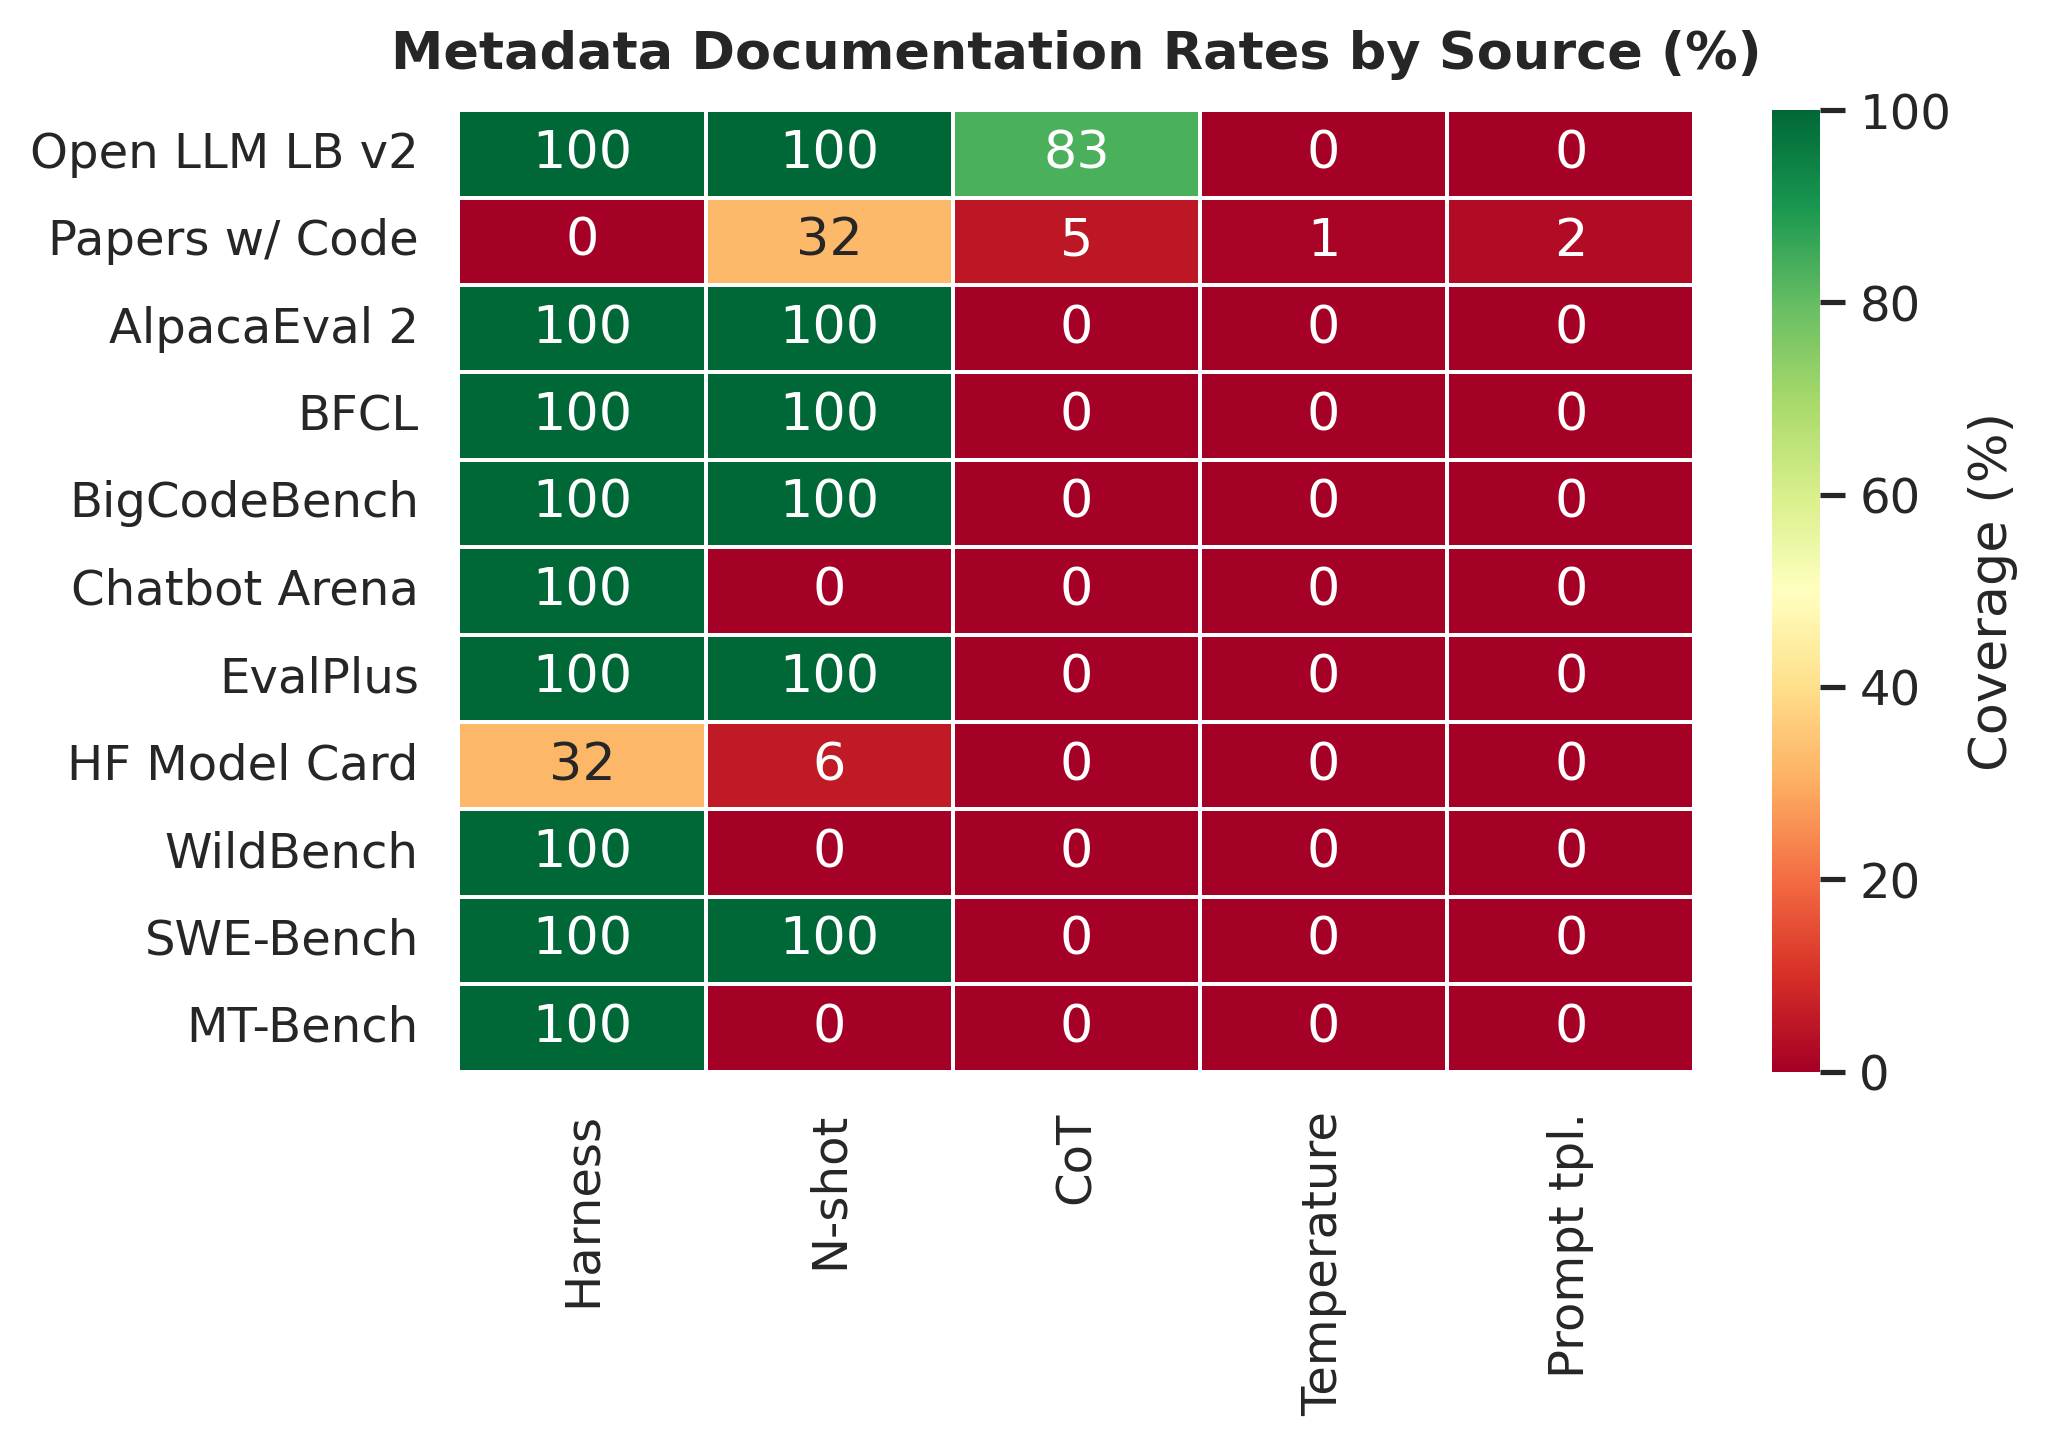
\includegraphics[width=\columnwidth]{figures/fig2_metadata_coverage.png}
\caption{Metadata documentation rates by source. Harness is
identified in most sources (98\% overall); n-shot is nearly
complete. Temperature and prompt template---the fields most critical
for understanding score differences---are virtually absent across
all sources.}
\label{fig:coverage}
\end{figure}

\subsection{Within-Source Score Conflicts}\label{sec:within}

Before examining cross-source comparisons, we first assess
consistency \emph{within} individual sources.

\paragraph{Data cleaning.}
An initial quality audit of the raw ingested data revealed
286~within-source conflicts---cases where the same
(model,~benchmark) pair appeared multiple times within a single
source with different scores. The dominant source was
\textbf{extraction errors} in Papers With Code (193~cases): model
parameter counts (e.g., 540 for PaLM~540B, 175 for GPT-3~175B)
leaked into score fields during automated table parsing.
A manual audit of 50~PWC records identified three distinct artefact types:
(a)~parameter-count leakage---model size suffixes (e.g., ``2.5B'') parsed
into \texttt{score} instead of \texttt{model\_info};
(b)~variant-tag leakage---model variant names (e.g., ``full'' from
``FiD-KD (full)'') routed to \texttt{generation\_args.prompt\_template};
and (c)~CoT-label misrouting---chain-of-thought descriptors parsed from
model-name parentheticals routed to \texttt{prompt\_template} instead of
\texttt{additional\_details.cot}, affecting at least 4~records in the
50-record sample.
Type~(a) accounts for the majority of the 193~automated conflicts;
types~(b) and~(c) were identified only through manual inspection and
would pass all automated checks, including schema validation.
We also
found 30~re-submission duplicates in Open LLM Leaderboard v2 and
63~minor stochastic variations ($|\Delta| < 1$) in WildBench. We
removed all extraction artefacts and duplicates through automated
cleaning (score-range filtering and deduplication), reducing the
PWC record count from 1,350 to 576. We then manually verified a
sample of PWC records against the original papers to confirm
that the remaining scores are correct.

\paragraph{Residual conflicts.}
After cleaning, only \textbf{1~within-source conflict} remains
(a minor score variation in HF Model Card), confirming that
extraction artefacts---not evaluation inconsistencies---were the
primary source of within-source noise. This cleaning step
demonstrates that even a schema-valid pipeline requires post-hoc
quality auditing to separate genuine evaluation results from
scraping artefacts---and strengthens the argument for mandatory
metadata documentation.
The audit also surfaces schema \emph{type} violations: at least one
PWC record contains \texttt{n\_shot}~=~``few'' (a string) rather
than an integer count, which passes JSON schema validation but
breaks numeric comparison---evidence that schema validity alone does
not guarantee semantic correctness.

\subsection{The Structural Wall (H2)}\label{sec:wall}

Cross-source comparison requires both \emph{benchmark overlap}
(two sources measure the same construct) and \emph{model overlap}
(two sources evaluate the same models). Figure~\ref{fig:overlap}
reveals that most source pairs fail one or both conditions.

\paragraph{Benchmark isolation.}
Of the $\binom{11}{2} = 55$ source pairs, only \textbf{4} share any
benchmarks at all:
\begin{itemize}[leftmargin=1.5em, itemsep=1pt]
\item HF Model Card $\times$ Open LLM LB v2: 5 benchmarks
\item HF Model Card $\times$ Papers w/ Code: 10 benchmarks
\item Open LLM LB v2 $\times$ Papers w/ Code: 5 benchmarks
\item EvalPlus $\times$ HF Model Card: 2 benchmarks
\end{itemize}
The remaining 51 pairs---including every pair involving AlpacaEval,
Chatbot Arena, BigCodeBench, MT-Bench, SWE-Bench, WildBench, or
BFCL---share \emph{zero} benchmarks. These 7 sources use
entirely unique benchmark suites (Arena ELO, WildBench score,
SWE-Bench-Verified, etc.) that no other source measures.

\paragraph{Model isolation.}
Even where benchmarks overlap, model overlap is sparse. The Jaccard
similarity between model sets is below 0.05 for all source pairs
except those involving the small HF Model Card source (11 models).
The Open LLM Leaderboard v2 evaluates 4,465 models, but only 18
of them also appear in Papers With Code for the same benchmarks.

Together, benchmark isolation and model isolation produce only
\textbf{16 collision pairs} from 29,331 records---a yield of
0.05\%. This is the structural wall: the evaluation landscape is
fragmented into non-overlapping silos, making systematic
cross-source comparison impossible at scale.

\paragraph{Is fragmentation structural or accidental?}
To test whether 16~collisions is unusually low, we run a Monte
Carlo simulation (1{,}000 iterations) under a null model where each
source randomly samples its model--benchmark pairs (preserving
observed source sizes) from the shared universe of 5,672 models and
180 benchmarks. The expected collision count is $67 \pm 8$
(mean $\pm$ SD; 95\% CI $[51, 84]$). The observed 16 yields
$z = -6.1$ (${p < 0.001}$; no simulated run produced $\leq 16$
collisions). Fragmentation is thus \emph{structural}---sources
systematically evaluate non-overlapping model sets---not an
artefact of small sample size.%
\footnote{The null model samples model--benchmark pairs uniformly
from the \emph{observed} universe of each source, preserving
per-source record counts. Earlier draft simulations that sampled
from the full Cartesian product (5,672$\times$180) produced higher
expected counts ($\sim$272); the current formulation is more
conservative because it respects the empirical sparsity of each
source's model and benchmark sets.}

\paragraph{Robustness to normalisation choices.}
The collision count depends on how model IDs and benchmark names are
normalised. Under \emph{strict} normalisation (exact lowercase
strings, no suffix stripping), the count drops to 6; under
\emph{loose} normalisation (additionally stripping version and
instruct/chat suffixes), the count remains 16. The qualitative
conclusion---fragmentation is extreme and attribution metadata is
missing---is invariant across this range.

\paragraph{Top-model disagreement.}
A practical consequence of structural isolation: for all 14
benchmarks shared by two or more sources, the ``top model'' differs
across every source pair. This occurs not because sources disagree on
rankings but because they evaluate non-overlapping model subsets---a
community practitioner looking for ``the best model on MMLU'' will
get a different answer depending on which source they consult, with
no way to reconcile the results.

\begin{figure}[t]
\centering
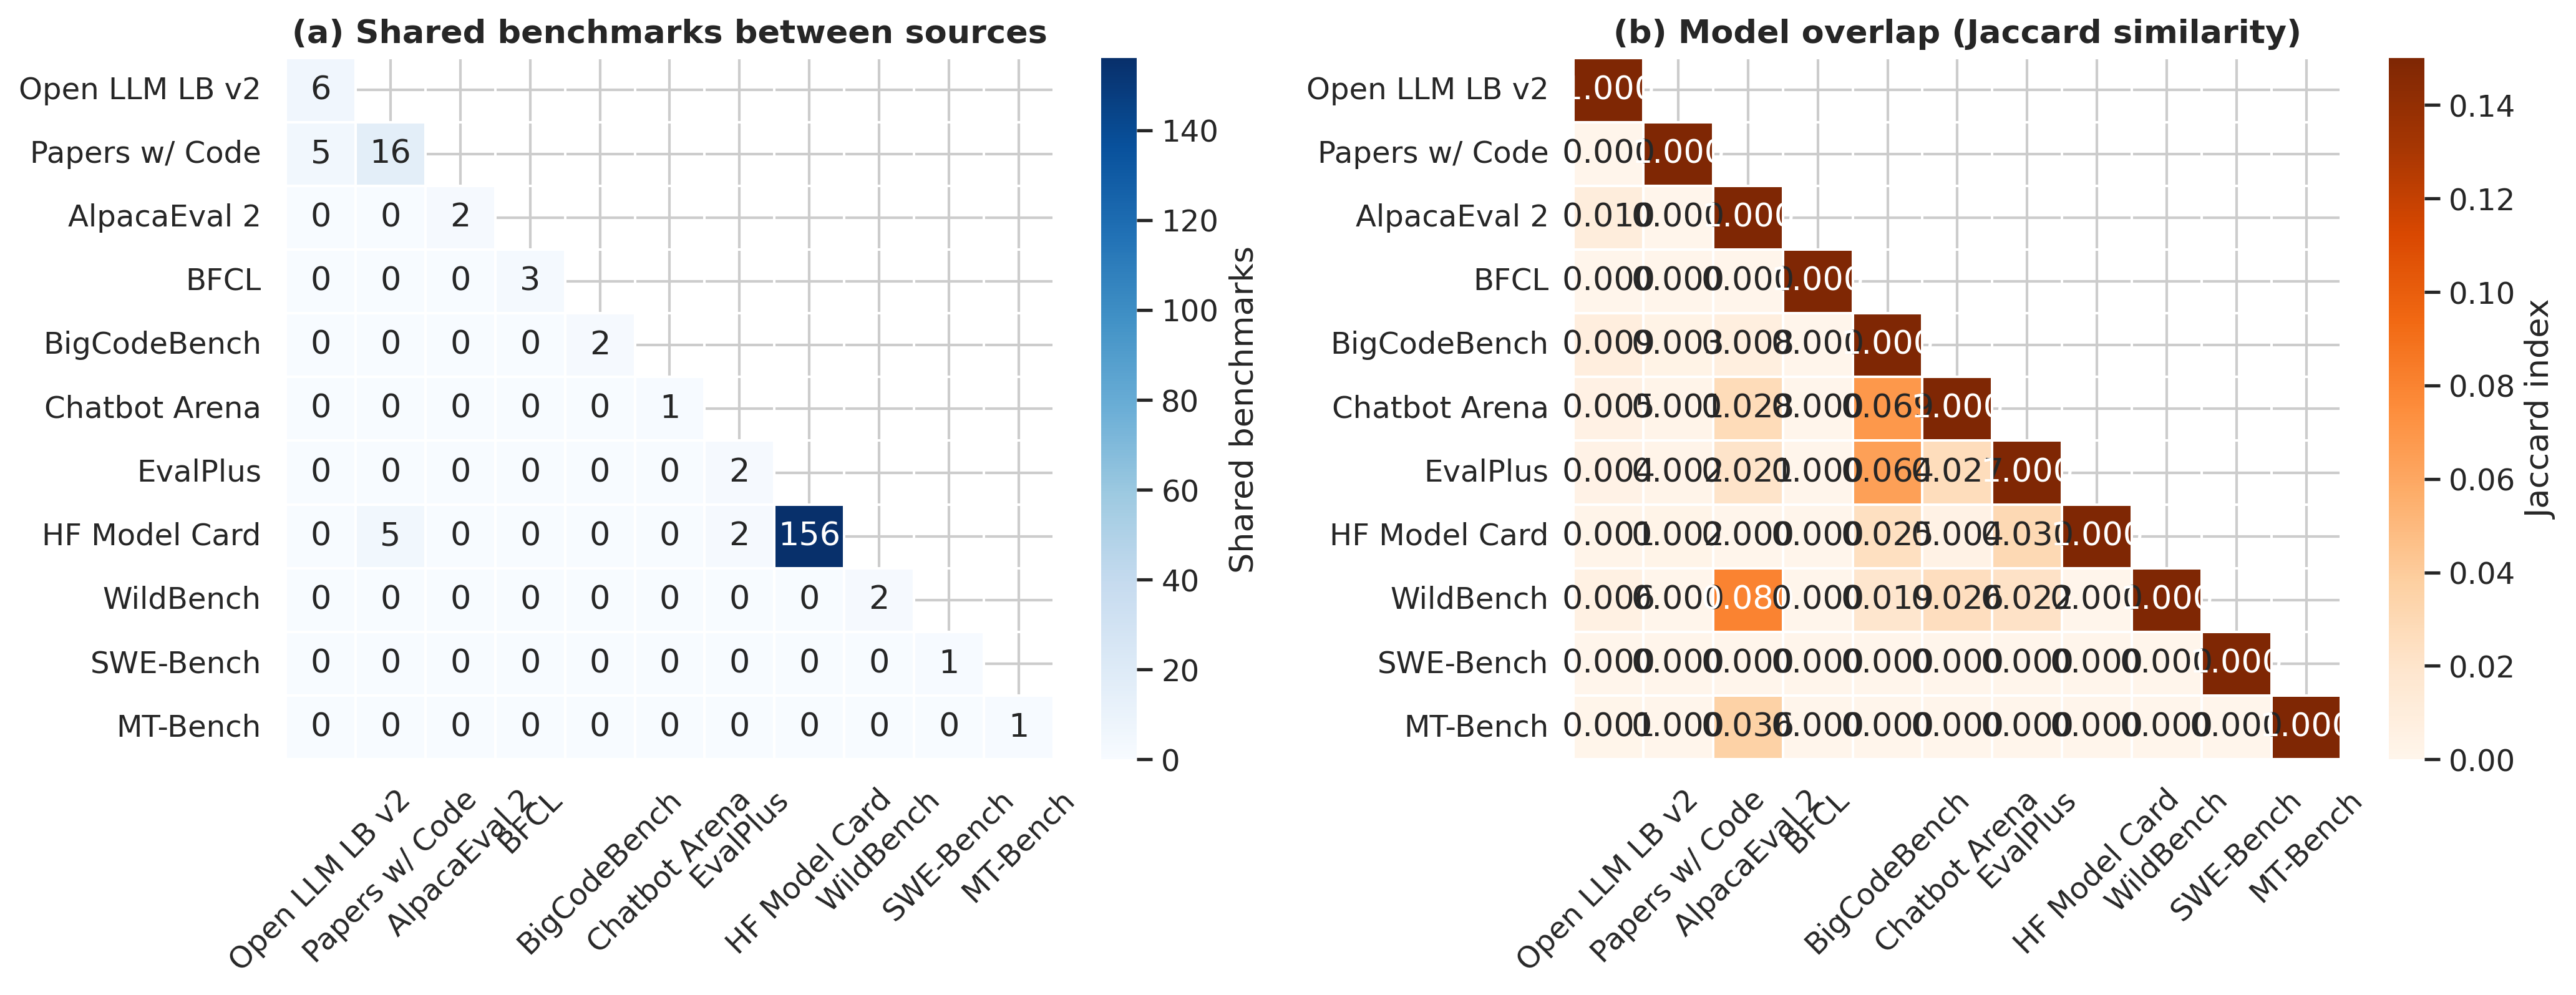
\includegraphics[width=\columnwidth]{figures/fig6_source_isolation.png}
\caption{The structural wall. \emph{Left}: shared benchmarks between
source pairs (most cells are zero). \emph{Right}: Jaccard index of
model overlap (nearly all below 0.05). Only 4 of 55 source pairs
share any benchmarks; only 16 collision pairs exist across the entire
29,331-record dataset.}
\label{fig:overlap}
\end{figure}

\subsection{Cross-Source Collisions (H3)}\label{sec:collisions}

Table~\ref{tab:collisions} lists all 16 collision pairs grouped by
benchmark. We separate these into \textbf{8~independent} pairs and
\textbf{8~likely copied} pairs, following the analysis in the
remainder of this section.

\paragraph{Total vs.\ independent collisions.}
Eight of the 16~pairs show $|\Delta| = 0.00$: the five
Tulu-3-70B-SFT collisions across BBH, GPQA, IFEval, MMLU-Pro, and
MuSR, and the three StarCoder2 base-model HumanEval+ pairs. These
are likely \emph{copied scores}---the HF Model Card authors
reproduced or transcribed scores from leaderboard sources rather
than running independent evaluations. Excluding these leaves
\textbf{8~genuinely independent collision pairs}, which constitute
our effective evidence base for cross-source analysis.

\paragraph{All collisions involve different harnesses.}
Every one of the 16 pairs compares a record evaluated with one
harness against a record from a different harness. This is not by
design---it is a consequence of intersection structure: the only
source pairs with both benchmark and model overlap
(HF Model Card~$\times$~Open LLM LB v2, HF Model Card~$\times$~%
EvalPlus) inherently use different evaluation frameworks.

\paragraph{Score gaps among independent pairs.}
Among the 8~independent pairs, the most extreme outlier is
Qwen2.5-72B-Instruct on GPQA: 16.67 (Open LLM LB v2, lm\_eval)
vs.\ 49.0 (Papers With Code, unknown harness)---a 32.3-point gap.
Two further outliers appear on MBPP+ ($|\Delta| = 3.9$) and
HumanEval+ ($|\Delta| = 3.0$), both comparing EvalPlus against
HF Model Card (transformers). The five Tulu-3-8B pairs show
$|\Delta| \leq 0.23$, consistent with genuine near-reproducibility
despite different harnesses (vllm vs.\ lm\_eval).

\paragraph{Attribution is blocked by missing metadata.}
For each of the 8~independent collision pairs, we categorised which
evaluation-context variables are documented in \emph{both} source
records. Table~\ref{tab:attribution} makes this concrete: temperature
and prompt template are unknown in every pair; n-shot is documented
in both sources for only 5 of 8~pairs; chain-of-thought status is
always missing on at least one side. Only harness identity is known
in both sources for 7 of 8~pairs (88\%)---but harness alone cannot
explain the score gaps, because the confounded variables (prompt
template, normalisation mode, answer extraction) are undocumented.
This means that even where cross-source comparisons are structurally
possible, \emph{every single one} is blocked from full attribution
by missing metadata.

\begin{table}[t]
\centering
\footnotesize
\setlength{\tabcolsep}{1.5pt}
\caption{Metadata availability per independent collision pair.
\cmark{} = documented in both sources; \ding{55} = missing in $\geq$1
source. Temperature and prompt template are absent in every pair.}
\label{tab:attribution}
\begin{tabular}{llccccc}
\toprule
\textbf{Model} & \textbf{Bench.} & \textbf{Harn.} & \textbf{Shots} & \textbf{CoT} & \textbf{Temp.} & \textbf{Prompt} \\
\midrule
Qwen2.5-72B-Inst. & GPQA    & \ding{55} & \ding{55}  & \ding{55} & \ding{55} & \ding{55} \\
SC2-15B-Inst.      & MBPP+   & \cmark    & \ding{55}  & \ding{55} & \ding{55} & \ding{55} \\
SC2-15B-Inst.      & HumanE+ & \cmark    & \ding{55}  & \ding{55} & \ding{55} & \ding{55} \\
Tulu-3-8B          & BBH     & \cmark    & \cmark     & \ding{55} & \ding{55} & \ding{55} \\
Tulu-3-8B          & GPQA    & \cmark    & \cmark     & \ding{55} & \ding{55} & \ding{55} \\
Tulu-3-8B          & IFEval  & \cmark    & \cmark     & \ding{55} & \ding{55} & \ding{55} \\
Tulu-3-8B          & MMLU-P  & \cmark    & \cmark     & \ding{55} & \ding{55} & \ding{55} \\
Tulu-3-8B          & MuSR    & \cmark    & \cmark     & \ding{55} & \ding{55} & \ding{55} \\
\midrule
\multicolumn{2}{l}{\emph{Known in both}} & 7/8 & 5/8 & 0/8 & 0/8 & 0/8 \\
\bottomrule
\end{tabular}
\end{table}

\begin{table}[t]
\centering
\footnotesize
\setlength{\tabcolsep}{2.5pt}
\caption{All 16 cross-source collision pairs, separated into
8~independent pairs (top) and 8~likely copied pairs (bottom).
Sources: OLv2 = Open LLM LB v2, HFM = HF Model Card, PWC =
Papers With Code, EP = EvalPlus. All pairs involve different
harnesses.}
\label{tab:collisions}
\begin{tabular}{llrrl}
\toprule
\textbf{Model (abbrev.)} & \textbf{Bench.} & $s_1$ & $s_2$ & $|\Delta|$ \\
\midrule
\multicolumn{5}{l}{\emph{Independent pairs}} \\
Qwen2.5-72B-Instruct    & GPQA       & 16.67 & 49.00 & 32.33 \\
StarCoder2-15B-Inst.     & MBPP+      & 65.10 & 61.20 &  3.90 \\
StarCoder2-15B-Inst.     & HumanE.+   & 60.40 & 63.40 &  3.00 \\
Tulu-3-8B                & BBH        & 16.86 & 16.67 &  0.19 \\
Tulu-3-8B                & GPQA       &  6.26 &  6.49 &  0.23 \\
Tulu-3-8B                & IFEval     & 82.55 & 82.67 &  0.12 \\
Tulu-3-8B                & MMLU-Pro   & 20.23 & 20.30 &  0.07 \\
Tulu-3-8B                & MuSR       & 10.52 & 10.45 &  0.07 \\
\midrule
\multicolumn{5}{l}{\emph{Likely copied (provenance inheritance)}} \\
Tulu-3-70B-SFT           & BBH        & 42.02 & 42.02 &  0.00 \\
Tulu-3-70B-SFT           & GPQA       & 12.64 & 12.64 &  0.00 \\
Tulu-3-70B-SFT           & IFEval     & 80.51 & 80.51 &  0.00 \\
Tulu-3-70B-SFT           & MMLU-Pro   & 40.27 & 40.27 &  0.00 \\
Tulu-3-70B-SFT           & MuSR       & 24.49 & 24.49 &  0.00 \\
StarCoder2-15B           & HumanE.+   & 37.80 & 37.80 &  0.00 \\
StarCoder2-3B            & HumanE.+   & 27.40 & 27.40 &  0.00 \\
StarCoder2-7B            & HumanE.+   & 29.90 & 29.90 &  0.00 \\
\bottomrule
\end{tabular}
\end{table}

\subsection{Case Study: The GPQA 32-Point Gap}\label{sec:casestudy}

The most striking collision is Qwen2.5-72B-Instruct on GPQA: the
Open LLM LB~v2 reports 16.67 (lm\_eval, 0-shot, CoT enabled)
while PWC reports 49.0 (harness unknown)---a 32.3-point gap. The
OLv2 record documents enough to identify that lm\_eval's GPQA
prompt template and answer normalisation produce lower scores than
alternative implementations, but the PWC record carries no harness,
prompt, or metric information, so the gap remains unexplained.
Contrast this with the five Tulu-3-8B pairs
($|\Delta| \leq 0.23$), where both sources document harness and
n-shot: the small residual is consistent with harness-internal
differences. The disparity between these two cases---metadata
absent $\Rightarrow$ attribution blocked vs.\ metadata partial
$\Rightarrow$ delta explainable---makes the coverage--attribution
gap tangible (Figure~\ref{fig:collisions}).

\begin{figure}[t]
\centering
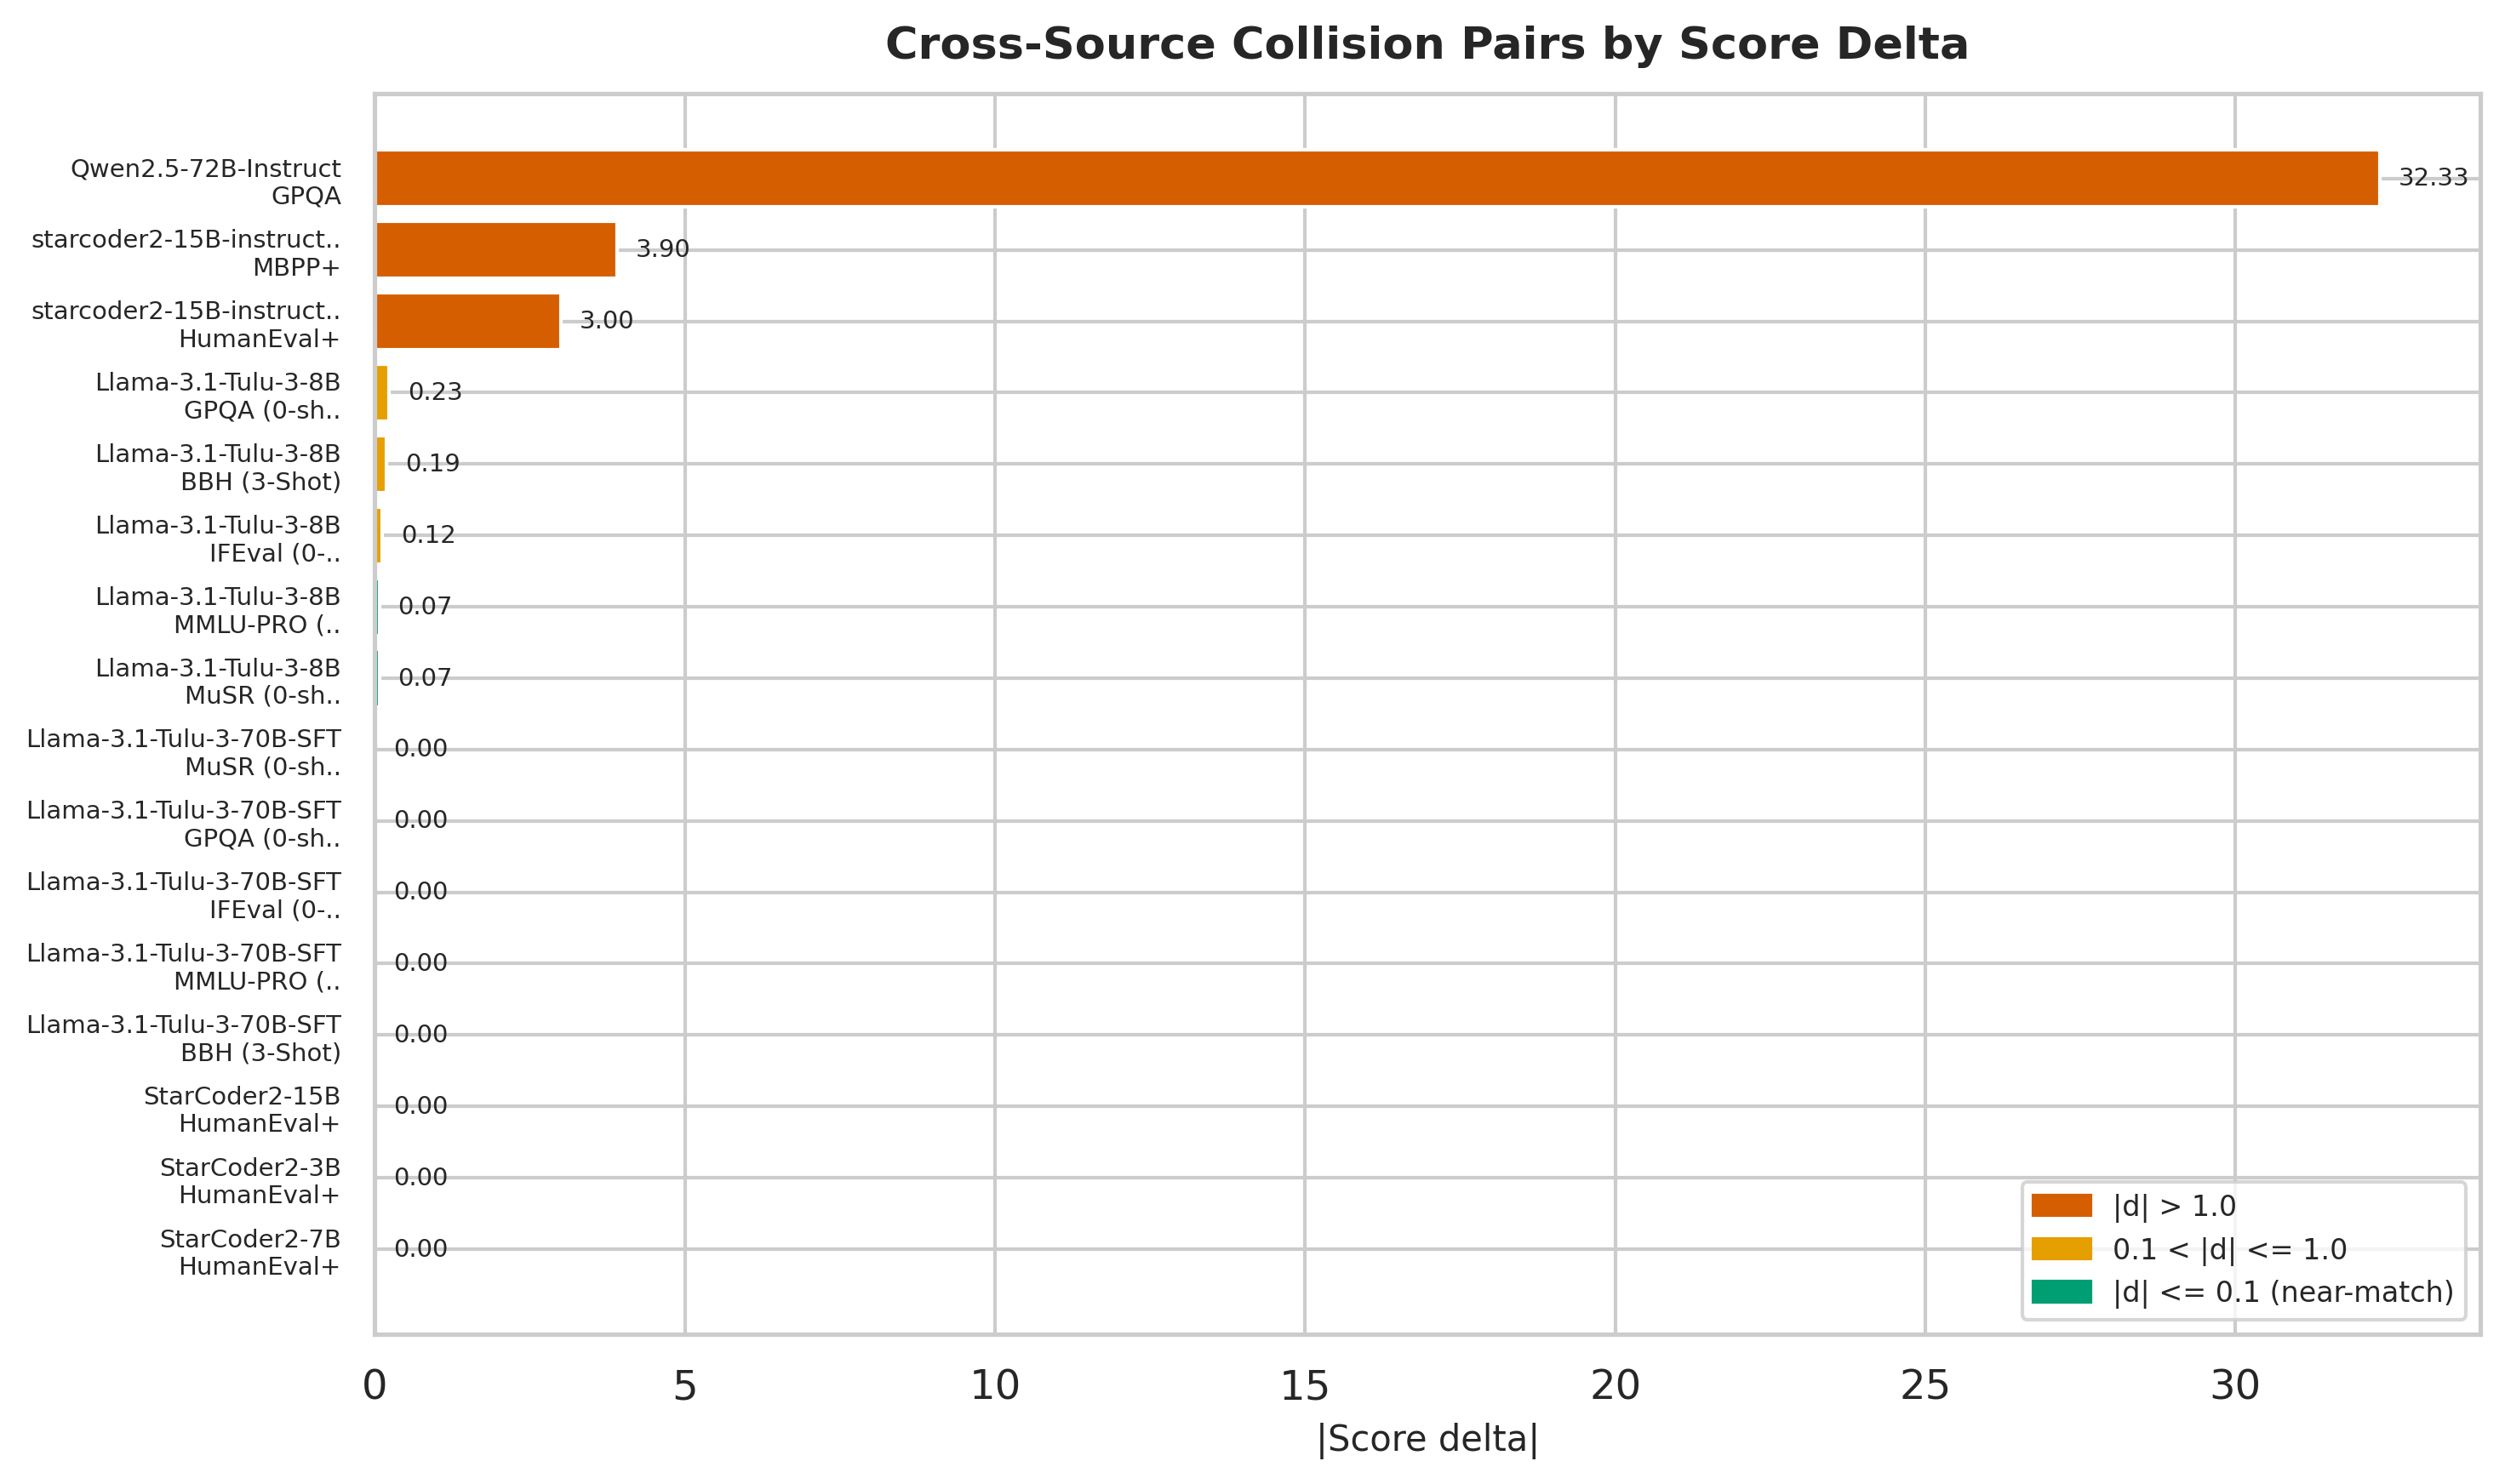
\includegraphics[width=\columnwidth]{figures/fig7_all_collisions.png}
\caption{All 16 cross-source collision pairs, ordered by absolute
delta. The GPQA collision (Qwen2.5-72B-Instruct, $|\Delta|=32.3$)
is a clear outlier. Colour encodes delta magnitude: red =
$|\Delta|>1$, orange = $|\Delta|>0.1$, green = $|\Delta|\leq0.1$.}
\label{fig:collisions}
\end{figure}

% ===================================================================
\section{Discussion}\label{sec:discussion}
% ===================================================================

\subsection{The Coverage--Attribution Gap}

Harness identity is known for 7~of~8 independent collision pairs
(88\%), yet temperature and prompt template are absent in
\emph{every} pair (Table~\ref{tab:attribution}). Even where
harness is documented, it is too coarse to explain score
gaps: attribution requires the fine-grained implementation
details---prompt format, normalisation mode, answer
extraction---that remain absent
\citep{biderman-2024-lessons, alzahrani-2024-benchmarks}.

\subsection{Structural Fragmentation}

The metadata gap is significant, but the structural wall
(\S\ref{sec:wall}) is arguably more fundamental. Even with perfect
metadata, only 16 collision pairs exist---24\% of the $67 \pm 8$
expected under random assignment ($z = -6.1$, $p < 0.001$)---because
leaderboards evaluate non-overlapping model--benchmark slices.
No amount of documentation can create cross-source comparisons
where the underlying data does not overlap.

\subsection{The Copied-Scores Problem}

Eight of our 16 collision pairs show $\Delta = 0.000$ (five
involving Tulu-3-70B-SFT across 5~benchmarks and three StarCoder2
base models on HumanEval+). These arise because the HF Model Card
source \emph{copied} scores from leaderboard sources rather than
running independent evaluations. The effective evidence base for
cross-source analysis is therefore \textbf{8~independent pairs},
not~16.

Identical scores can thus indicate either (i)~genuine
reproducibility or (ii)~provenance inheritance. Distinguishing
these requires a provenance-tracking field not currently in the
EEE schema. We propose \texttt{provenance\_link} for v0.3:
a URI pointing to the original evaluation run
(e.g., \url{https://huggingface.co/spaces/open-llm-leaderboard/results})---making
score inheritance machine-detectable, a need underscored by the
8~of~16 collision pairs (50\%) in our dataset that show
$\Delta=0.00$ and are likely copied.

\subsection{Recommendations}

Based on our coverage audit, we propose three tiers of action:

\paragraph{For leaderboard maintainers.}
Every published benchmark result should document at minimum:
(1)~the \textbf{prompt template} or a canonical identifier
(currently $<$0.1\% coverage---the most critical gap);
(2)~the \textbf{temperature} ($<$0.1\%); and
(3)~the \textbf{harness version}, not just the framework name
but the specific commit hash or release, since defaults change
between releases. Leaderboards could auto-generate EEE records
with these fields populated at evaluation time.

\paragraph{For model developers.}
Authors should ship EEE-formatted evaluation files alongside model
cards, replacing unstructured tables with machine-parseable records
that carry full evaluation context.

\paragraph{For platform adoption.}
If platforms like Open LLM Leaderboard~v2 or Chatbot Arena
natively emitted EEE-formatted records---embedding prompt template,
temperature, and harness version at evaluation time---the metadata
gap would close for new evaluations. The EEE schema is designed to
lower the adoption barrier: a leaderboard could emit one JSON
record per evaluation run with minimal pipeline changes.

\paragraph{For schema designers.}
We propose two extensions for EEE v0.3:
(i)~\texttt{scoring\_mode} (enum: greedy generation, log-likelihood,
execution-based); and (ii)~\texttt{provenance\_link} (URI pointing
to the original source when scores are copied rather than
independently evaluated). Our released dataset uses EEE v0.2.1;
future schema revisions will be accompanied by migration tooling
and the dataset will be updated accordingly.

\subsection{Ecosystem-Level Findings}
\label{sec:shared_task}

The ingestion process surfaced~three schema--ecosystem mismatches:
(i)~\texttt{eval\_library.version} is ``unknown'' in all
29,331~records---no source publishes the harness commit hash,
making it impossible to determine whether two records using the
same harness name share the same implementation
\citep{biderman-2024-lessons};
(ii)~scoring mode (log-likelihood vs.\ generation vs.\ execution)
is not a first-class schema field, forcing it into free-text
\texttt{additional\_details}; and
(iii)~provenance inheritance is undetectable---8~of~16 collision
pairs (50\%) carry $\Delta=0.00$ and are likely copied
(\S\ref{sec:collisions}), but no \texttt{provenance\_link} field
exists to flag this.

\subsection{Threats to Validity}\label{sec:threats}

\paragraph{Source composition.}
Our dataset is heavily skewed: Open LLM Leaderboard~v2 contributes
91\% of records. As Table~\ref{tab:ablation} shows, removing it
changes n-shot coverage from 96.7\% to 62.2\% and chain-of-thought
from 76.3\% to 1.1\%. The qualitative conclusion---temperature and
prompt template are essentially absent---is stable across all
ablations, but the ecosystem-wide shots and CoT figures depend on
this single source.

\paragraph{Within-source noise (PWC).}
Papers With Code required significant data cleaning
(\S\ref{sec:within}): we removed 774~records containing extraction
artefacts and duplicates. Even after cleaning, PWC has the weakest
metadata coverage (harness unknown, n-shot at 32\%). The single
most dramatic collision pair (GPQA, $|\Delta|=32.3$) depends on
PWC---a limitation we flag for transparency. We manually verified
a sample of remaining PWC records against original papers.
Additionally, at least 2~PWC records (GAL~1.3B and Gopher~1.4 on
TruthfulQA) report scores on a 0--1 fractional scale rather than
the 0--100 percentage scale used by all other records; such
unit-scale inconsistencies are not detectable by range-based sanity
checks alone and require normalisation verification against the
citing paper.

\paragraph{Normalisation sensitivity.}
Our collision detection uses rule-based string normalisation for
model IDs and benchmark names. Varying the strictness yields a
range of 6 (exact lowercase) to 16 (our default) collision pairs;
the qualitative conclusions are invariant
(\S\ref{sec:wall}).

\paragraph{Within-harness vs.\ cross-source analysis.}
All 16~collision pairs involve different harnesses, because the
only source pairs with model--benchmark overlap inherently use
different evaluation frameworks. We therefore cannot quantify
within-harness sensitivity from our data. Our analysis is
exclusively cross-source: it characterises the structure of the
public evaluation ecosystem rather than measuring the causal
effect of individual evaluation-context variables.

\paragraph{Collision pair count.}
With only 16~pairs (8~independent, 8~likely copied), no statistical
inference about score distributions is warranted. Our results are
descriptive: they characterise the current state of a rapidly
evolving ecosystem.

% ===================================================================
\section{Conclusion}\label{sec:conclusion}
% ===================================================================

We tested four hypotheses about the LLM evaluation ecosystem
using 29,331 records from 11~sources (5,672 models, 180 benchmarks)
standardised via the EEE schema. All four are confirmed:

\begin{enumerate}[leftmargin=2em, itemsep=1pt]
\item \textbf{H1 (Metadata gap) confirmed}: prompt template and
  temperature are documented in fewer than 0.1\% of records---and
  even the nominal $<$0.1\% figure is a false positive (100\% of
  non-null \texttt{prompt\_template} values are extraction
  artefacts). N-shot (96.7\%) and harness (98\%) appear
  well-covered, but these figures are inflated by a single source
  contributing 91\% of records; excluding it drops n-shot to 62\%
  and CoT to 1\% (\S\ref{sec:coverage}).
\item \textbf{H2 (Structural fragmentation) confirmed}: only
  16 cross-source collision pairs exist---24\% of the $67 \pm 8$
  expected under random assignment ($z = -6.1$, $p < 0.001$)---because sources evaluate non-overlapping model--benchmark
  combinations (\S\ref{sec:wall}).
\item \textbf{H3 (Attribution failure) confirmed}: among the
  8~independent collision pairs, all involve different harnesses
  and all lack the metadata needed to explain score gaps of up to
  32.3~points (\S\ref{sec:collisions}).
\item \textbf{H4 (Pipeline fragility) confirmed}: 43\% of raw
  Papers With Code records (774 of 1,350) were extraction
  artefacts or duplicates that passed schema validation but
  required post-hoc auditing to detect. Three distinct artefact
  types were identified; two (variant-tag leakage and CoT-label
  misrouting) are invisible to automated range checks
  (\S\ref{sec:within}).
\end{enumerate}

To move from detecting differences to explaining them, the
community needs both better metadata documentation (prompt template,
temperature, harness version) and deliberate overlap in evaluation
scope. We release our dataset, pipeline (${\sim}4{,}900$~LOC), and
analysis code under CC-BY-4.0.

% ===================================================================
\section*{Limitations}
% ===================================================================

The following limitations are not covered by the threats to validity
analysis in \S\ref{sec:threats}.

\paragraph{Schema gaps.}
The EEE schema (v0.2.1) does not enforce several factors known to
affect scores: normalisation mode, pass@$k$, decoding limits, and
LLM-as-judge configuration. These can be recorded in free-form
\texttt{additional\_details} but are not validated or analysed.

\paragraph{Manual audit.}
We performed a targeted manual audit of Papers With Code records,
verifying sampled scores against the original papers to confirm
semantic correctness after automated data cleaning. However,
we did not conduct a full systematic audit across all 11~sources.
While all 29,331~records pass schema validation, we cannot report
precision or recall for individual metadata fields across the full
dataset. A comprehensive random-sample audit of, e.g.,
50--100~records per source is important future work.

\paragraph{Temporal snapshot.}
Our dataset reflects a single snapshot of each source. Leaderboards
are updated continuously; model cards are revised; Papers With Code
tables grow. The structural wall and coverage rates may evolve as
sources expand their model--benchmark scope.

% ===================================================================
\section*{Ethics Statement}
% ===================================================================

All data in this study consists of publicly available evaluation
scores and metadata from open leaderboards, model cards, and
structured paper-results archives. No model outputs, training data,
or personally identifiable information was collected or analysed.

Our findings quantify structural fragmentation and missing metadata
in the evaluation ecosystem. We emphasise that these results are
intended to \emph{improve} evaluation practices---by motivating
better documentation and deliberate cross-source overlap---not to
dismiss leaderboards, which remain the primary mechanism for
transparent, community-wide model comparison.

Papers With Code records were obtained by scraping structured
evaluation tables that aggregate third-party paper results. We use
these data for meta-scientific analysis under fair-use principles,
cite original papers where available, and release our derived
dataset under CC-BY-4.0.

%% -------------------------------------------------------------------
\bibliography{refs,custom}
\bibliographystyle{acl_natbib}
%% -------------------------------------------------------------------

\appendix

\section{Supplementary Figures}\label{app:figures}

\begin{figure*}[t]
\centering
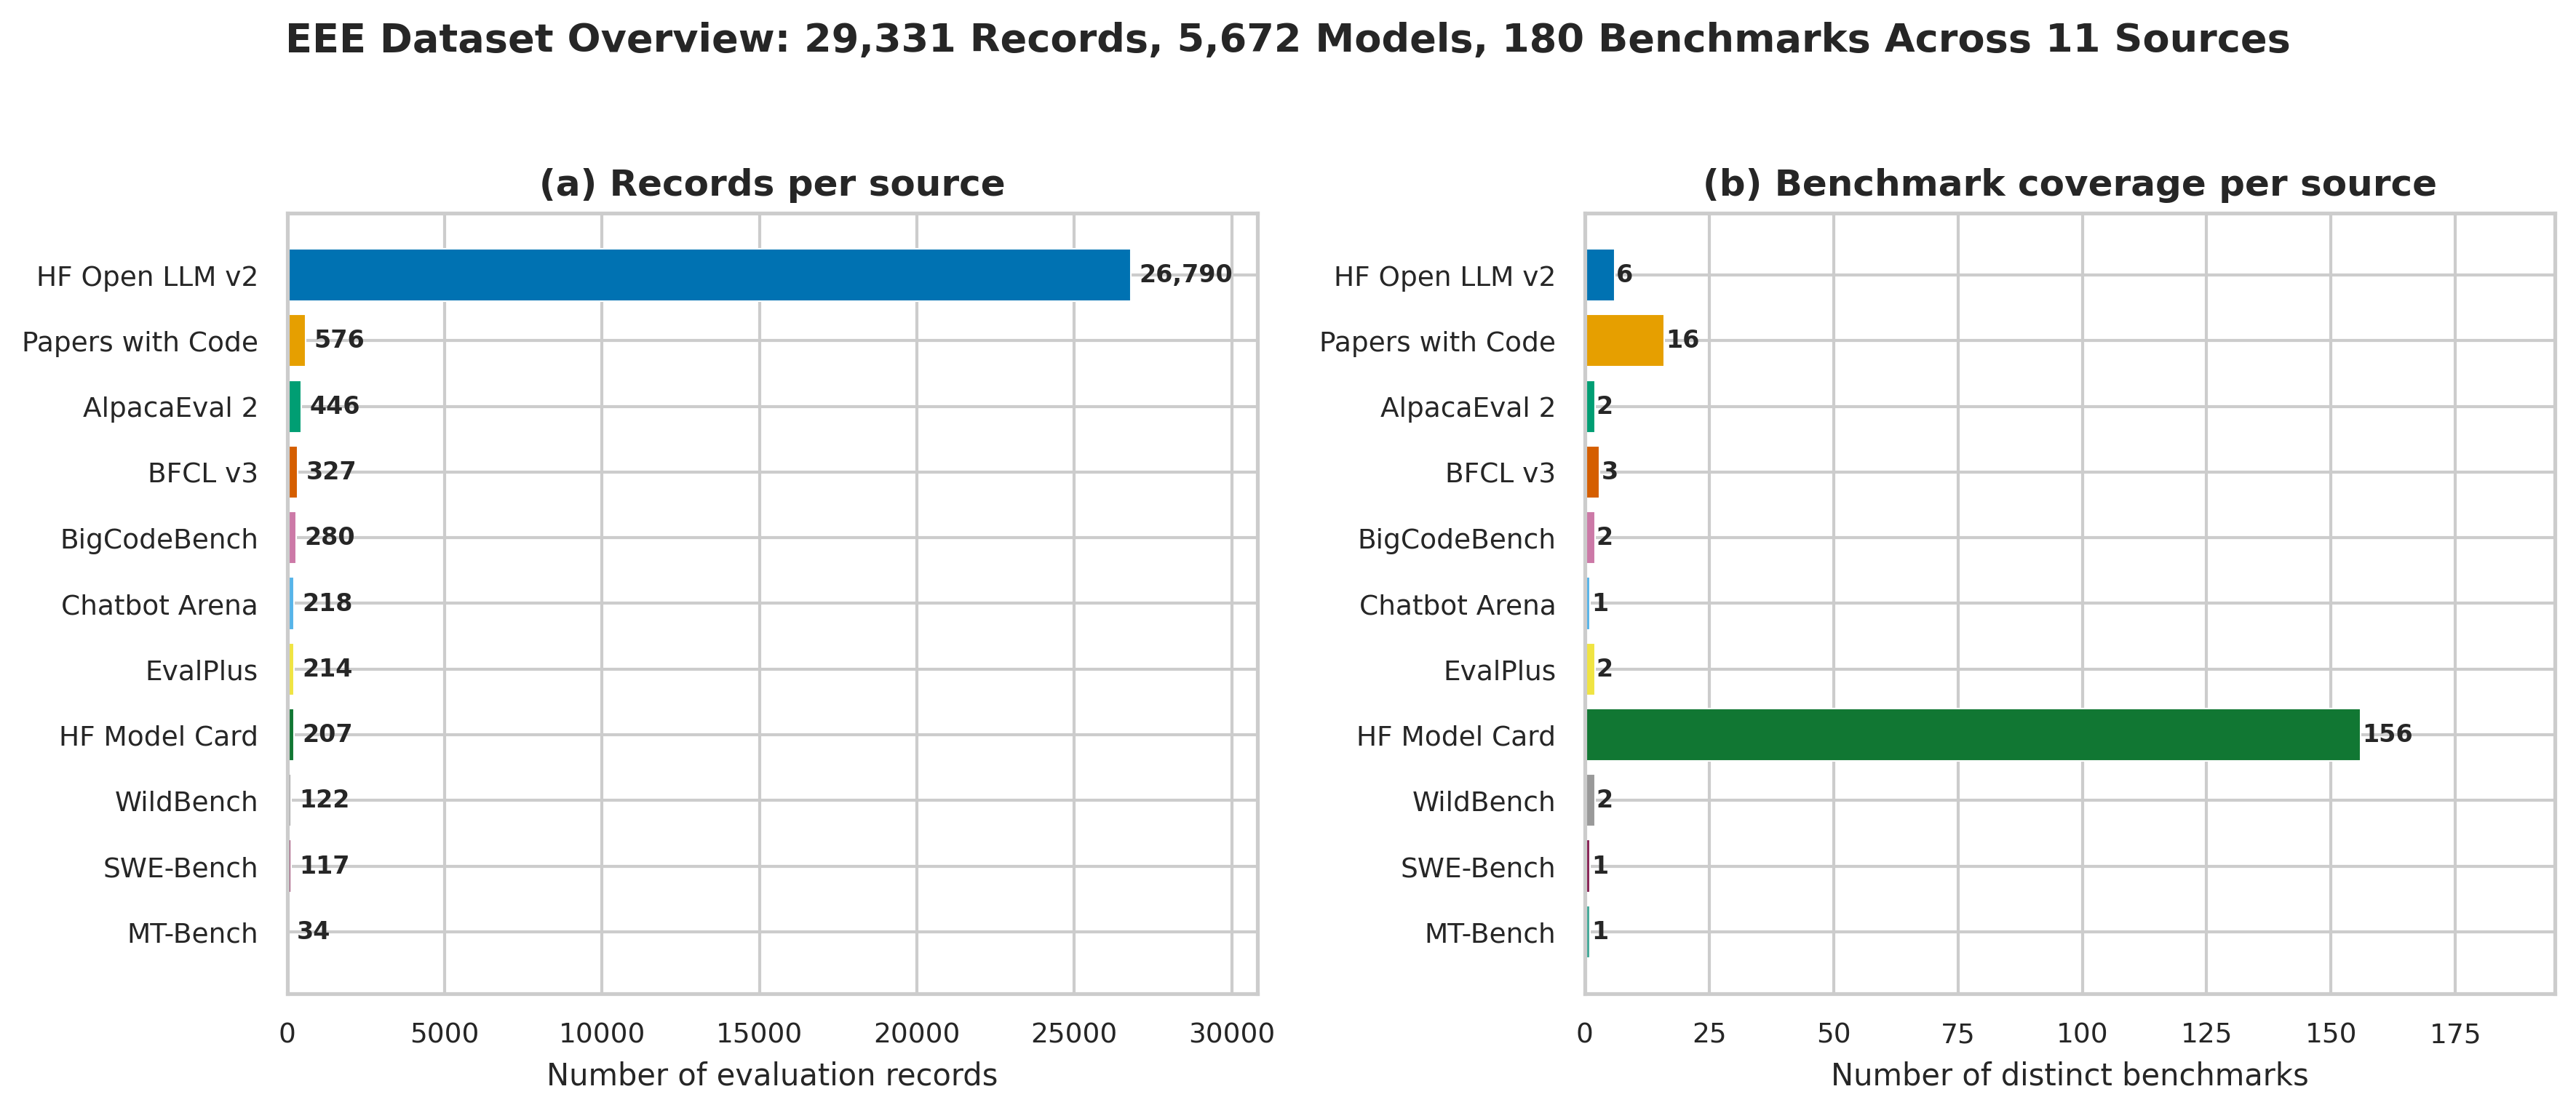
\includegraphics[width=\textwidth]{figures/fig4_dataset_composition.png}
\caption{Dataset composition by source. \emph{Left}: total evaluation
records (log-scaled axis). \emph{Centre}: unique models per source.
\emph{Right}: unique benchmarks per source. The Open LLM Leaderboard
v2 dominates in records and models; HF Model Card is the outlier in
benchmark diversity (156 benchmarks from only 11 models).}
\label{fig:composition}
\end{figure*}

\begin{figure*}[t]
\centering
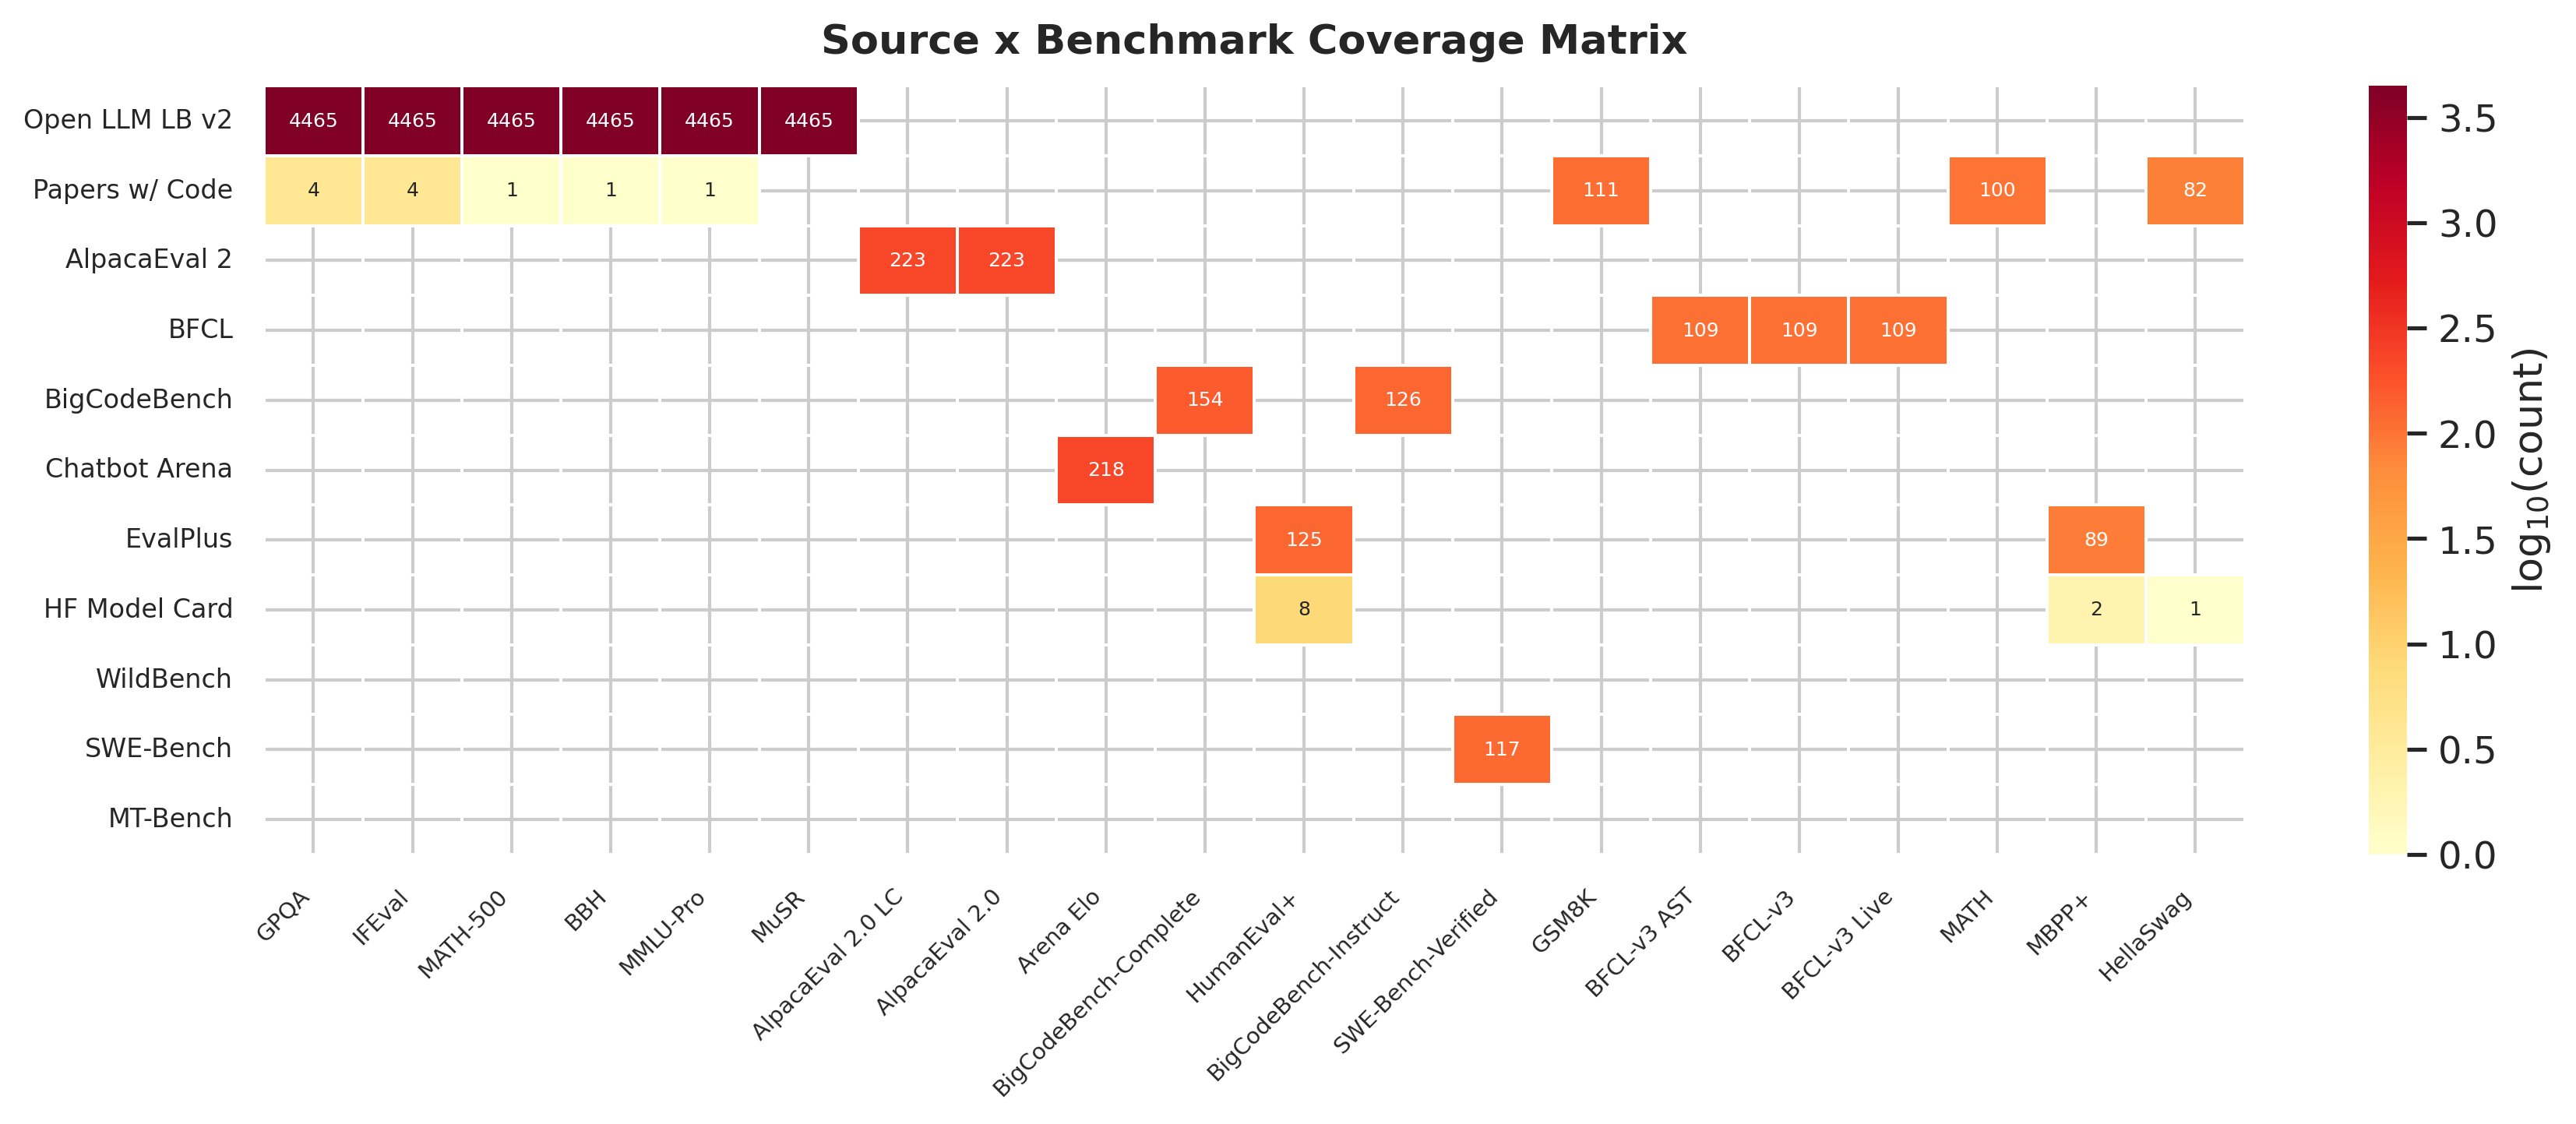
\includegraphics[width=\textwidth]{figures/fig1_source_benchmark_matrix.png}
\caption{Evaluation records per source--benchmark pair (log$_{10}$
scale). Each row is a source; each column is a benchmark (top~20 by
record count). Blank cells indicate zero coverage. The sparsity of
this matrix---most cells are zero---drives the shortage of
cross-source collision pairs.}
\label{fig:matrix}
\end{figure*}

\section{Converter Architecture}\label{app:converters}

The pipeline comprises two converter families:

\paragraph{Framework adapters (2,465 LOC).}
Four adapters parse evaluation log files from established harnesses:
lm-evaluation-harness (JSON result files), HELM (scenario outputs),
Inspect~AI (eval logs), and a common base class providing shared
field extraction and normalisation.

\paragraph{Leaderboard scrapers (2,456 LOC).}
Seven scrapers handle API and dataset ingestion: HF Open LLM
Leaderboard~v2 (HuggingFace Datasets API), AlpacaEval~2.0,
BigCodeBench, Chatbot Arena (public leaderboard tables),
EvalPlus (HuggingFace dataset), BFCL (gorilla API), and
SWE-Bench/WildBench/MT-Bench (HuggingFace spaces).

Benchmark name canonicalisation uses a manually curated mapping
table. For Papers With Code, we map 16 PWC dataset identifiers to
canonical benchmark names (e.g., ``mmlu'' $\rightarrow$ ``MMLU'').
For HF Model Cards, we rely on structured YAML
\texttt{model-index} fields.

\end{document}
